\chapter{\IfLanguageName{dutch}{Stand van zaken}{State of the art}}%
\label{ch:stand-van-zaken}

% Tip: Begin elk hoofdstuk met een paragraaf inleiding die beschrijft hoe
% dit hoofdstuk past binnen het geheel van de bachelorproef. Geef in het
% bijzonder aan wat de link is met het vorige en volgende hoofdstuk.

% Pas na deze inleidende paragraaf komt de eerste sectiehoofding.

% Commentaar = ctrl + t

%Dit hoofdstuk bevat je literatuurstudie. De inhoud gaat verder op de inleiding, maar zal het onderwerp van de bachelorproef *diepgaand* uitspitten. De bedoeling is dat de lezer na lezing van dit hoofdstuk helemaal op de hoogte is van de huidige stand van zaken (state-of-the-art) in het onderzoeksdomein. Iemand die niet vertrouwd is met het onderwerp, weet nu voldoende om de rest van het verhaal te kunnen volgen, zonder dat die er nog andere informatie moet over opzoeken \autocite{Pollefliet2011}.
%
%Je verwijst bij elke bewering die je doet, vakterm die je introduceert, enz.\ naar je bronnen. In \LaTeX{} kan dat met het commando \texttt{$\backslash${textcite\{\}}} of \texttt{$\backslash${autocite\{\}}}. Als argument van het commando geef je de ``sleutel'' van een ``record'' in een bibliografische databank in het Bib\LaTeX{}-formaat (een tekstbestand). Als je expliciet naar de auteur verwijst in de zin (narratieve referentie), gebruik je \texttt{$\backslash${}textcite\{\}}. Soms is de auteursnaam niet expliciet een onderdeel van de zin, dan gebruik je \texttt{$\backslash${}autocite\{\}} (referentie tussen haakjes). Dit gebruik je bv.~bij een citaat, of om in het bijschrift van een overgenomen afbeelding, broncode, tabel, enz. te verwijzen naar de bron. In de volgende paragraaf een voorbeeld van elk.
%
%\textcite{Knuth1998} schreef een van de standaardwerken over sorteer- en zoekalgoritmen. Experten zijn het erover eens dat cloud computing een interessante opportuniteit vormen, zowel voor gebruikers als voor dienstverleners op vlak van informatietechnologie~\autocite{Creeger2009}.
%
%Let er ook op: het \texttt{cite}-commando voor de punt, dus binnen de zin. Je verwijst meteen naar een bron in de eerste zin die erop gebaseerd is, dus niet pas op het einde van een paragraaf.
%
%\begin{figure}
%  \centering
%  
\includegraphics[width=0.8\textwidth]{grail.jpg}
%  \caption[Voorbeeld figuur.]{\label{fig:grail}Voorbeeld van invoegen van een figuur. Zorg altijd voor een uitgebreid bijschrift dat de figuur volledig beschrijft zonder in de tekst te moeten gaan zoeken. Vergeet ook je bronvermelding niet!}
%\end{figure}
%
%\begin{listing}
%  \begin{minted}{python}
%    import pandas as pd
%    import seaborn as sns
%
%    penguins = sns.load_dataset('penguins')
%    sns.relplot(data=penguins, x="flipper_length_mm", y="bill_length_mm", hue="species")
%  \end{minted}
%  \caption[Voorbeeld codefragment]{Voorbeeld van het invoegen van een codefragment.}
%\end{listing}
%
%\lipsum[7-20]
%
%\begin{table}
%  \centering
%  \begin{tabular}{lcr}
%    \toprule
%    \textbf{Kolom 1} & \textbf{Kolom 2} & \textbf{Kolom 3} \\
%    $\alpha$         & $\beta$          & $\gamma$         \\
%    \midrule
%    A                & 10.230           & a                \\
%    B                & 45.678           & b                \\
%    C                & 99.987           & c                \\
%    \bottomrule
%  \end{tabular}
%  \caption[Voorbeeld tabel]{\label{tab:example}Voorbeeld van een tabel.}
%\end{table}

% Inleiding

Hier komt een inleiding...


% Deel 1 - stress en burn-out bij twintigers

\section{Stress en burn-out bij twintigers}
\label{sec:burnout-bij-twintigers}

\subsection{Wat is een burn-out?}
\label{subsec:wat-is-burnout}

\vspace{1em}

Hoewel de term \textit{burn-out} in het dagelijkse taalgebruik steeds frequenter voorkomt, bestaat er vaak onduidelijkheid over de precieze betekenis en afbakening ervan. Een concrete definiëring is dan ook noodzakelijk om het begrip binnen dit onderzoek correct te situeren.

\vspace{1em}

Volgens de elfde herziening van de \acrlong{icd} (\acrshort{icd}-11) van de \acrshort{who} wordt burn-out sinds 2019 omschreven als een syndroom dat het gevolg is van chronische werk gerelateerde stress die onvoldoende werd aangepakt \autocite{world-health-organization-who-2019}. Hoewel het begrip werd opgenomen in de \acrshort{icd}, wordt het niet geclassificeerd als een medische aandoening, maar als een werkgerelateerd fenomeen.

\vspace{1em}

Dit beroepsgerelateerd syndroom wordt gekenmerkt door drie kerncomponenten:
\begin{itemize}
    \item \textbf{Uitputting}: een aanhoudend gevoel van vermoeidheid of mentale uitputting;
    \item \textbf{Cynisme}: een toenemende mentale afstand tot het werk, of een negatieve en cynische houding tegenover de functie;
    \item \textbf{Verminderd gevoel van effectiviteit}: een verminderd gevoel van bekwaamheid en effectiviteit in het uitvoeren van professioneel werk.
\end{itemize}

\vspace{1em}

Ook \textcite{MonteroMarin2011} omschreven burn-out reeds als een syndroom ten gevolge van chronische werkstress, gekenmerkt door uitputting, cynisme en verminderde professionele effectiviteit. Zij benadrukken dat burn-out niet bij iedereen op dezelfde manier tot uiting komt en onderscheiden drie subtypen: \textit{“frenetic”}, \textit{“underchallenged”} en \textit{“worn-out”}.

\vspace{1em}

\subsubsection{Frenetic burnout}
\label{subsubsec:frenetic}

Een hectische burn-out wordt door \textcite{MonteroMarin2011} beschreven als gekenmerkt door passie, ambitie en een sterke betrokkenheid, waarbij personen veel tijd en energie in hun werk steken. Dit kan leiden tot gevoelens van overbelasting en uiteindelijk tot uitputting.

\vspace{1em}

\subsubsection{Underchallenged burnout}
\label{subsubsec:underchallenged}

Bij dit type burnout, aldus \textcite{MonteroMarin2011}, ervaren personen te weinig uitdaging of persoonlijke ontwikkeling in hun werk. Dit gaat vaak gepaard met verveling en onverschilligheid, wat kan resulteren in cynisme. Daarnaast kan de oppervlakkige of repetitieve uitvoering van taken leiden tot een verminderd gevoel van effectiviteit.

\vspace{1em}

\subsubsection{Worn-out burnout}
\label{subsubsec:worn-out}

Wanneer personen het gevoel hebben weinig controle over hun werkzaamheden te hebben en onvoldoende erkenning krijgen voor hun inspanningen, ontstaat het laatste subtype, zoals beschreven door \textcite{MonteroMarin2011}. Dit kan leiden tot passief gedrag, een verminderd gevoel van effectiviteit, versterkt cynisme en bijdragen aan mentale uitputting, vooral door aanhoudende stress en gevoelens van machteloosheid.

\vspace{1em}



\subsection{De huidige burn-out cijfers onder de loep}
\label{subsec:burnout-cijfers}

\vspace{1em}

Recente cijfers van het \textcite{RIZIV2023_invaliditeit_burnout} tonen aan dat burn-out steeds vaker voorkomt in onze samenleving. Eind 2023 werden maar liefst \textbf{45.771} personen gerapporteerd als langdurig arbeidsongeschikt door burn-out, een stijging van bijna 71\% ten opzichte van 26.835 gevallen in 2018. Binnen deze algemene stijging valt vooral de jongste leeftijdscategorie op. Het aantal burn-outgevallen bij volwassenen onder de 30 jaar verdubbelde van 825 in 2018 naar 1.707 in 2023, een \textbf{toename} van \textbf{107\%}, wat de maatschappelijke relevantie van burn-out onder twintigers extra benadrukt \autocite{RIZIV2023_invaliditeit_burnout}.

\begin{figure}[H]
    \centering
    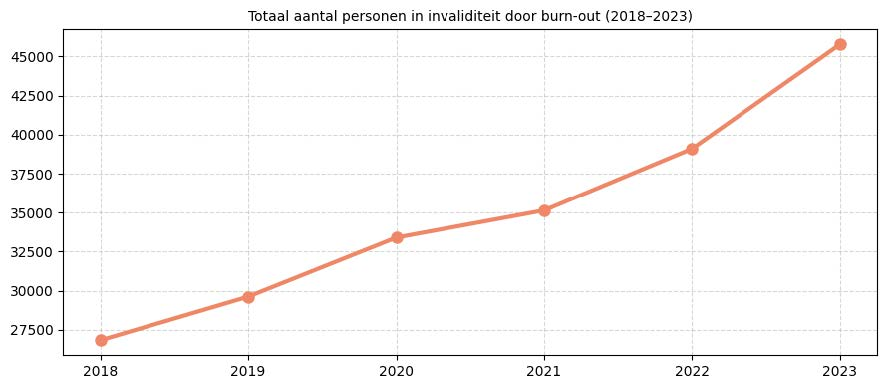
\includegraphics[width=\textwidth]{../graphics/burnout-cijfers-2}
    \caption{Totale evolutie van het aantal personen in invaliditeit door burn-out in België tussen 2018 en 2023 (bron: \autocite{RIZIV2023_invaliditeit_burnout}).}
\end{figure}

\vspace{1em}

\begin{figure}[H]
    \centering
    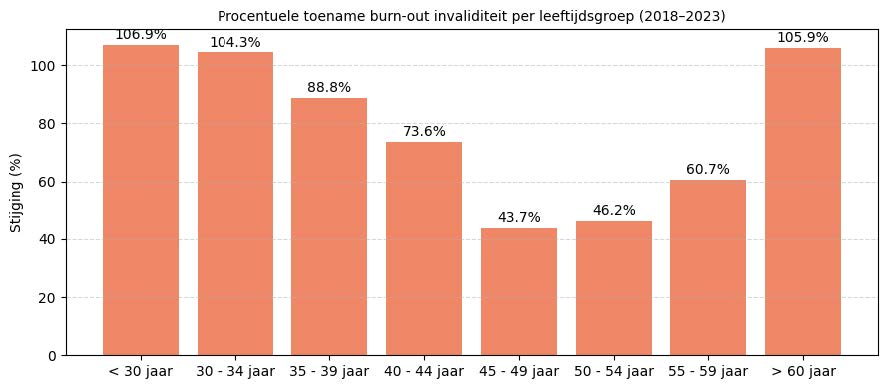
\includegraphics[width=\textwidth]{../graphics/burnout-cijfers-1}
    \caption{\label{fig:procent-stijging-burnout}Procentuele toename van burn-out gerelateerde invaliditeit per leeftijdsgroep tussen 2018 en 2023. Deze verticale staafdiagram maakt duidelijk welke leeftijdsgroepen relatief het sterkst gestegen zijn, met name de groep <30 jaar (bron: \autocite{RIZIV2023_invaliditeit_burnout}).}
\end{figure}

\vspace{1em}
\vspace{1em}
\vspace{1em}
\vspace{1em}

\textcite{SERV2024_werkbaarwerk} bevestigt via hun Vlaamse Werkbaarheidsmonitor daarbij de omvang van het probleem: maar liefst \textbf{13\%} van de jonge werknemers (18-35 jaar) rapporteert symptomen van burn-out, terwijl 35,9\% werkstressklachten ervaart. Dit toont aan dat naast langdurige arbeidsongeschiktheid, ook beginnende burn-outklachten aanzienlijk aanwezig zijn bij jonge werknemers.



\subsection{Kenmerken van de doelgroep}
\label{subsec:kenmerken-generatieZ}

\vspace{1em}

Burn-out is een begrip dat leeft binnen tal van leeftijdscategorieën. In dit onderzoek ligt de focus echter op de groep jonge volwassenen, aangezien uit de voorgaande sectie “Huidige burn-out cijfers onder de loep” blijkt dat bij hen de burn-outcijfers het sterkst stijgen. Om zo specifiek mogelijk te werk te gaan, wordt de doelgroep herleid tot één generatie: \textbf{generatie Z}.

\vspace{1em}

Voordat we ingaan op de risicofactoren die deze generatie kwetsbaar maken voor burn-out, is het eerst essentieel om de kenmerken van generatie Z in kaart te brengen. Dit zowel op het vlak van normen, waarden als van hun gedrag en houding op de werkvloer. 

\vspace{1em}

\subsubsection{Demografische en algemene kenmerken}
\label{subsubsec:demografic-z}

\vspace{1em}

Generatie Z, ook wel gen Z genoemd, is een verzameling aan individuen die geboren zijn tussen 1995 en 2012 \autocite{annerixt-2025}. Het grootste kenmerk aan deze groep, ook wel 14-31 jarigen, is dat ze opgegroeid zijn in een volledig digitale, verbonden wereld waardoor ze al vaak omschreven worden als \textbf{“digital natives”} \autocite{Peredy2024}. Zo zijn ze volgens \textcite{Peredy2024} technisch zeer vaardig, gebruiken ze intensief digitale tools (\textit{zoals sociale media}) en communiceren ze vaak via visuele middelen (\textit{zoals GIFs, memes en korte video’s}). Daarnaast staat deze generatie bekend om haar zeer inclusieve en diverse mindset, sterke maatschappelijke betrokkenheid en ondernemingszin \autocite{Peredy2024}.

\vspace{1em}

\subsubsection{Persoonlijkheidskenmerken}
\label{subsubsec:perskenmerken-z}

\vspace{1em}

Volgens \textcite{annerixt-2025} wordt deze generatie gekenmerkt door een opvallende combinatie van ambitie, perfectionisme, creativiteit en een sterke werkethiek. Ze streven ernaar om uit te blinken in wat ze doen en leggen daarbij veel nadruk op kwaliteit en persoonlijke prestaties. Tegelijkertijd hechten ze veel waarde aan zelfexpressie en persoonlijke ontwikkeling, wat hun verlangen naar autonomie en het vormen van hun eigen identiteit benadrukt \autocite{Zahra2025}.

\vspace{1em}

Ondanks deze sterkte kanten vertoont deze groep ook zwakkere en soms tegenstrijdige eigenschappen. Zo kunnen ze kwetsbaar, zelfgericht en gevoelig voor stress zijn \autocite{annerixt-2025}. Deze combinatie van hoge ambitie en kwetsbaarheid maakt volgens \textcite{Zahra2025} dat individuele erkenning van hun prestaties voor hen van groot belang is.

\vspace{1em}

Samengevat vormt deze generatie een mix van gedrevenheid en creativiteit, gecombineerd met een opvallende gevoeligheid, waarbij persoonlijke ontwikkeling en erkenning centraal staan in hun dagelijks handelen en keuzes.

\vspace{1em}

\subsubsection{Psychologische basisbehoeften op de werkvloer}
\label{subsubsec:psychbehoeften-z}

\vspace{1em}

Steeds meer individuen van generatie Z betreden de werkvloer. Het wordt alsmaar duidelijker dat deze generatie bepaalde psychologische basisbehoeften heeft ontwikkeld die hun functioneren en welzijn sterk beïnvloeden. Volgens \textcite{annerixt-2025} zijn drie kernbehoeften hierbij essentieel: autonomie, competentie en verbondenheid.

\begin{itemize}
    \item \textbf{Autonomie}: het vermogen om zelf keuzes te kunnen maken en controle te hebben over de toegewezen taken;
    \item \textbf{Competentie}: het ervaren van succes en effectiviteit op het werk;
    \item \textbf{Verbondenheid}: ondanks een zekere neiging tot zelfgerichtheid blijft samenwerking, sociale steun en erkenning binnen hun netwerk van groot belang.
\end{itemize}

\vspace{1em}

Naast deze basisbehoeften toont generatie Z een duidelijke focus op mentaal welzijn \autocite{annerixt-2025}. Factoren zoals een gezonde werk-privé balans, erkenning, flexibiliteit en mogelijkheden voor persoonlijke groei zijn voor hen cruciaal. Wanneer deze behoeften onvoldoende vervuld worden, kan dit leiden tot een verhoogd risico op stress, futloosheid en zelfs burn-out \autocite{Zahra2025}. Dit benadrukt dat organisaties die generatie Z optimaal willen ondersteunen niet alleen moeten inzetten op prestaties, maar ook op een omgeving die persoonlijke ontwikkeling en welzijn actief stimuleert.

\vspace{1em}

\subsubsection{Werkhouding, verwachtingen en stressfactoren}
\label{subsubsec:werkhouding-z}

\vspace{1em}

Volgens \textcite{Zahra2025} streeft generatie Z naar zinvol werk, flexibiliteit en mogelijkheden voor persoonlijke groei. Ze willen niet enkel functioneren als “tandwieltjes” in een organisatie, maar vinden het belangrijk dat hun werk bijdraagt aan een groter doel en dat ze zich continu kunnen ontwikkelen.

\vspace{1em}

Echter, door hun ambitieus en perfectionistisch karakter, worden ze regelmatig geconfronteerd met hoge prestatiedruk. De constante blootstelling aan digitale informatie en sociale media zorgt ervoor dat velen zich bijna continu “aan” voelen staan, waardoor het moeilijk is om te ontspannen en echt los te koppelen van werk en verplichtingen \autocite{annerixt-2025}. Bovendien maakt deze generatie zich constant zorgen over hun toekomst, carrièrekansen, financiële situatie, gezondheid, het klimaat en politieke ontwikkelingen, wat bijdraagt aan verhoogde stressniveaus \autocite{annerixt-2025}. 

\vspace{1em}

Hoewel hun technologische vaardigheden de productiviteit en efficiëntie kunnen verhogen, kan overmatig gebruik van digitale tools en sociale media juist leiden tot mentale overbelasting en extra stress \autocite{Zahra2025}. Dit maakt duidelijk dat generatie Z niet alleen behoefte heeft aan uitdagend en betekenisvol werk, maar ook aan een werkomgeving die hen ondersteunt bij het reguleren van werkdruk en het behouden van hun mentale welzijn.

\vspace{1em}



\subsection{Specifieke risicofactoren bij generatie Z}
\label{subsec:risicofactoren-twintigers}



% Deel 2 - digitalisering en cognitieve belasting

\section{Digitalisering en cognitieve belasting}
\label{sec:digitalisering-cognitief}

\subsection{De impact van digitalisering op mentale gezondheid}
\label{subsec:impact-digitalisering}

\subsection{Information overload en permanente bereikbaarheid}
\label{subsec:info-overload}

\subsection{Technostress}
\label{subsec:technostress}

\subsection{Online vigilance}
\label{subsec:online-vigilance}

% Deel 3 - Preventie- en behandelingsstrategieën bij stress en burn-out

\section{Preventie- en behandelingsstrategieën bij stress en burn-out}
\label{sec:preventie-behandeling}

\subsection{Primaire, secundaire en tertiaire preventie}
\label{subsec:preventie-types}

\subsection{Cognitieve-gedragstherapie}
\label{subsec:cgt}

\subsubsection{Rational Emotive Behavior Therapy}
\label{subsubsec:rebt}

\subsubsection{Cognitieve gedragstherapie (CGT)}
\label{subsubsec:cgt-therapie}

\subsection{Psycho-educatie}
\label{subsec:psycho-educatie}

\subsection{Mindfulness}
\label{subsec:mindfulness}

% Deel 4 - Digitale interventies voor mentale gezondheid

\section{Digitale interventies voor mentale gezondheid}
\label{sec:digitale-interventies}

\subsection{E-health en m-health toepassingen}
\label{subsec:e-m-health}

\subsection{Effectiviteit van mentale gezondheidsapps}
\label{subsec:effectiviteit-apps}

\subsection{Engagement en retentieproblematiek}
\label{subsec:engagement-retentie}

\subsection{Kritieken op bestaande mentale gezondheidsapps}
\label{subsec:kritieken-apps}

% Deel 5 - UX- en ontwerpprincipes voor mentale rust

\section{UX- en ontwerpprincipes voor mentale rust}
\label{sec:ux-ontwerp}

\subsection{UI-elementen en cognitieve belasting}
\label{subsec:ui-cognitieve-belasting}

\subsection{Calm design en minimalisme}
\label{subsec:calm-design}

\subsection{Personalisatie en autonomie}
\label{subsec:personalisatie-autonomie}

\subsection{Gamification: ondersteunend of stresserend?}
\label{subsec:gamification}

\subsection{Notificatiestrategieën}
\label{subsec:notificaties}

% Deel 6 - Technologieselectie

\section{Technologieselectie}
\label{sec:technologieselectie}
